\documentclass[a4paper]{article}

% Includes packages relevant to Senior Lab

% character set specifications
\usepackage[english]{babel}
\usepackage[utf8]{inputenc}

% increased vertical spacing for tables
\newcommand\topVspace{\rule{0pt}{2.6ex}}      
\newcommand\bottomVspace{\rule[-1.2ex]{0pt}{0pt}} 

% extra unicode characters
\DeclareUnicodeCharacter{3BC}{\(\mu\)}
\DeclareUnicodeCharacter{3C1}{\(\rho\)}
\DeclareUnicodeCharacter{2080}{\(_0\)}
\DeclareUnicodeCharacter{2081}{\(_1\)}
\DeclareUnicodeCharacter{2082}{\(_2\)}
\DeclareUnicodeCharacter{3B5}{\(\epsilon\)}
\DeclareUnicodeCharacter{3B1}{\(\alpha\)}

% SI Units
\usepackage{siunitx}

% extra SI units
\DeclareSIUnit\gauss{G}

% enable scientific notation
\sisetup{scientific-notation = engineering, exponent-to-prefix}

% draw pretty lines
\usepackage{tikz}
\usetikzlibrary{datavisualization}
\usepackage{circuitikz}

% manual tabbing
\setlength{\parindent}{0pt}
\def\qq{\qquad}

% include graphics
\usepackage{graphicx}

% increased control over figure placement
\usepackage{float}

% box answers
\usepackage{tcolorbox}

% enable multiple section levels
\usepackage{titlesec}

% define `\subsubsubsection` command
\titleclass{\subsubsubsection}{straight}[\subsection]
\newcounter{subsubsubsection}[subsubsection]
\renewcommand\thesubsubsubsection{\thesubsubsection.\arabic{subsubsubsection}}
\titleformat{\subsubsubsection}
        {\normalfont\normalsize\bfseries}{\thesubsubsubsection}{1em}{}
\titlespacing*{\subsubsubsection}
{0pt}{3.25ex plus 1ex minus .2ex}{1.5ex plus .2ex}
\setcounter{secnumdepth}{4}

% get align environment (among other things)
\usepackage{amsmath}

% bold in math mode
\usepackage{bm}

% get \mathbb (among other things)
\usepackage{amssymb}

\usepackage{array}

% plotting
\usepackage{pgfplots}

% enable external references
\usepackage{hyperref}

% include code
\usepackage[cache=false]{minted}
\setminted{linenos, frame=lines, texcomments}

% adjust margins of individual pages (for shoving figures into place)
\usepackage{changepage}

% rotate figures
\usepackage{rotating}


\usepackage{subfigure}

\usepackage{caption}
\renewcommand{\thetable}{\arabic{section}.\arabic{table}}
\newcommand\T{\rule{0pt}{2.6ex}}       % Top strut
\newcommand\B{\rule[-1.2ex]{0pt}{0pt}} % Bottom strut

\title{PHY 4210-01 Senior Lab \\Lab C1:  Mathematical Models of Chaotic Physical Systems }

\author{Sarah Arends \\
        Jacquelyne Miksanek \\
        Ryan Wojtyla \\ \\
        Instructor: Gus Azelis}

\date{\today}

\begin{document}
\maketitle

\begin{abstract}
%physics of experiment
%apparatus used
%what was measured
%Results
\qq Chaotic behavior was studied by creating mathematical models and altering key parameters. A simple chaotic model was then observed by measuring time intervals of droplet formation from a leaking faucet. A small change in initial conditions can equate to much larger changes in the behavior of a system.

\end{abstract}

\newpage

\tableofcontents

\newpage

\section{The Logistic Equation}
\qq A population model can be represented with equation \ref{eq:log}, where $0<x_n<1$ and $r<4$. These parameters can be modified to observe the onset of chaotic behavior. The period doubling and chaotic regions will be investigated.

\begin{equation}
x_{n+1} = r x_n (1-x_n)
\label{eq:log}
\end{equation}

\subsection{Period Doubling Region of the Logistic Equation}
% progression of x_n for perioud doubling
\qq A period doubling region exists for $r<3.56994$. Plots of $x_n$ versus $x$ are produced for $0<r<3.56994$. Figure \ref{pdoub1} shows this behavior for a range of $r$ values. For $r<3$, the set of $x_n$ converge to a particular value, although they may fluctuate for the first few iterations. Around $r=3$ the values of $x_n$ oscillate between two values, as seen in figure \ref{pdoub1}. Around $r=3.5$, the values of $x_n$ begin oscillating between 4 values. This exhibits the period doubling region.

% xn vs n graph
\begin{figure}[H]
\centering
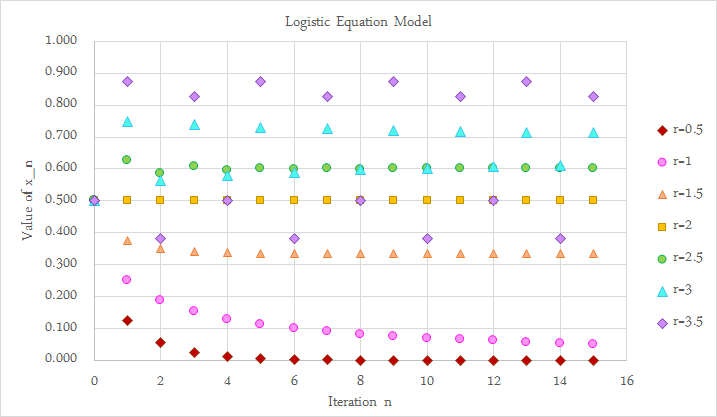
\includegraphics[width=1\textwidth]{pdoub.png}
\captionof{figure}{Series of $x_n$ vs $x$ for varying parameters $r<3.56994$. Plots of $x_n$ versus $x$ are produced for initial condition $x_0=0.5$. This is the period doubling region.}
\label{pdoub1}
\end{figure}

\subsection{Chaotic Region of the Logistic Equation}
% Part b and c
\qq A chaotic region occurs for $r>3.56994$. Plots of $x_n$ versus $x$ are produced for this region and graphed in figure \ref{chaos1}. The distributions for each $r$ value appear seemingly random because, although the system is deterministic, it is very sensitive to small changes.

% xn vs n graph, varying r
\begin{figure}[H]
\centering
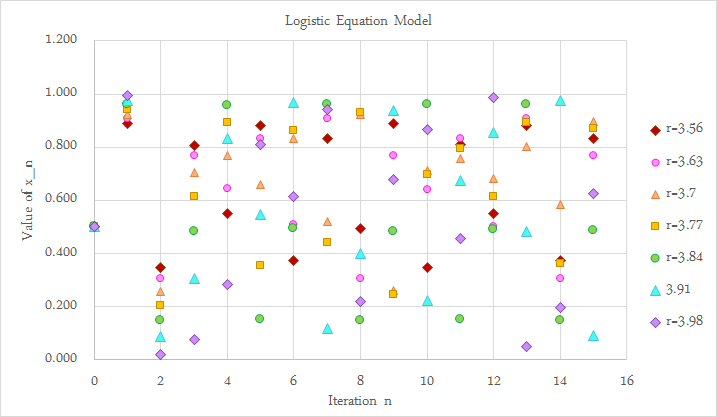
\includegraphics[width=1\textwidth]{chaos1.png}
\captionof{figure}{Series of $x_n$ vs $x$ for varying parameters $r>3.56994$. Plots of $x_n$ versus $x$ are produced for initial condition $x_0=0.5$. This is the chaotic region.}
\label{chaos1}
\end{figure}

% varying x_0
The behavior of $x_n$ is investigated by varying the initial condition $x_0$ by small amounts. A small change in this initial condition will produce even greater variations as $n$ gets large. For the range of $n$ values shown in figure \ref{varyx0}, the percent change in $x_n$ values was computed between the series corresponding to initial conditions $x_0=0.8$ and $x_0=0.801$. The percent change was minimized for the zeroth iteration, at $0.125\%$. The difference was at a maximum of $437\%$ for the fourteenth iteration, and the change was closest to $1\%$ for the eighth iteration.

% xn vs n graph, varying x0
\begin{figure}[H]
\centering
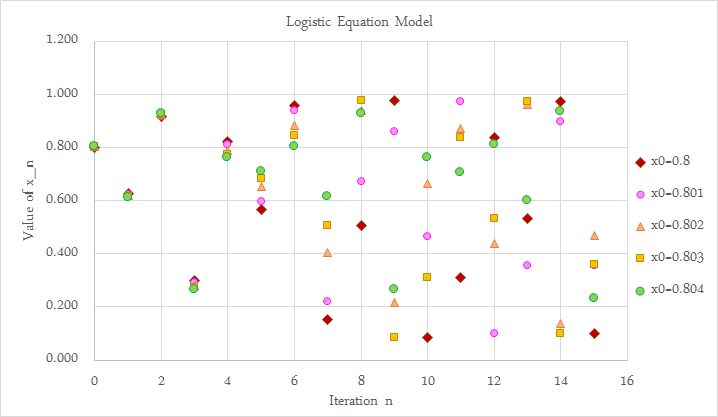
\includegraphics[width=1\textwidth]{varyx0.png}
\captionof{figure}{Series of $x_n$ vs $x$ for varying initial conditions $x_0$. Plots of $x_n$ versus $x$ are produced for $r=3.91$, which falls in the chaotic region.}
\label{varyx0}
\end{figure}

\section{Lyapunov Experiments}
% Part d and e

\subsection{Water Drop Experiment}
% words on what we did

% plots 1 and 2
\begin{figure}[H]
\centering
\begin{minipage}{.5\textwidth}
  \centering
  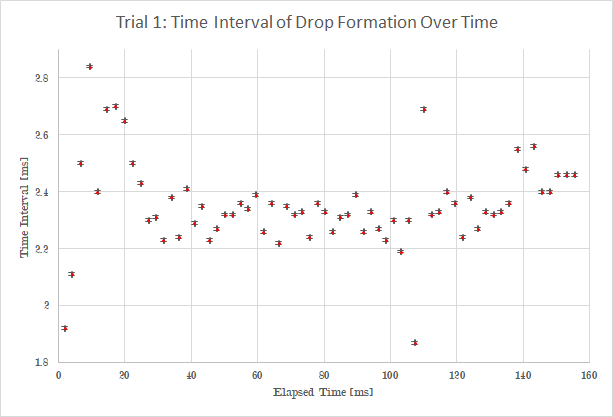
\includegraphics[width=\linewidth]{sink1.png}
  \captionof{figure}{sink1}
  \label{fig:test1}
\end{minipage}%
\begin{minipage}{.5\textwidth}
  \centering
  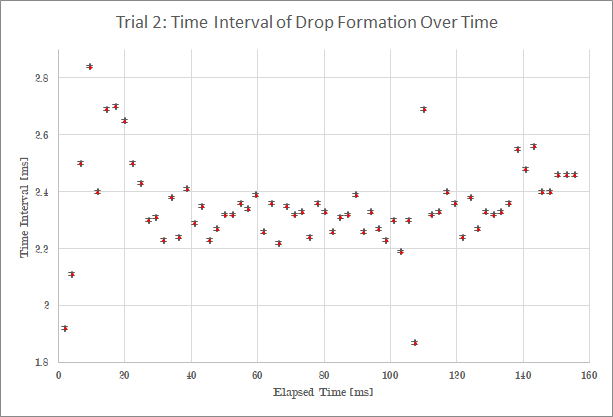
\includegraphics[width=\linewidth]{sink2.png}
  \captionof{figure}{sink2}
  \label{fig:test2}
\end{minipage}
\end{figure}

% plots 3 and 4
\begin{figure}[H]
\centering
\begin{minipage}{.5\textwidth}
  \centering
  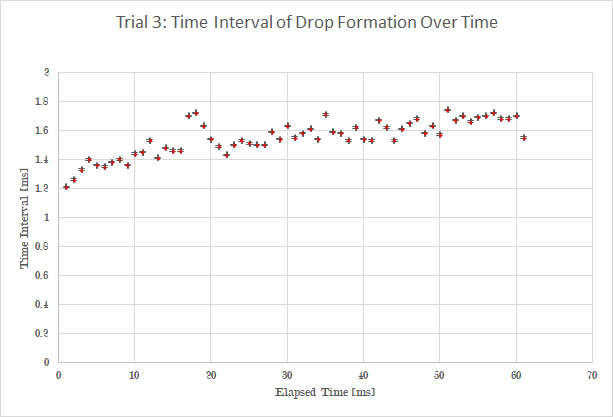
\includegraphics[width=\linewidth]{sink3.png}
  \captionof{figure}{sink3}
  \label{fig:test1}
\end{minipage}%
\begin{minipage}{.5\textwidth}
  \centering
  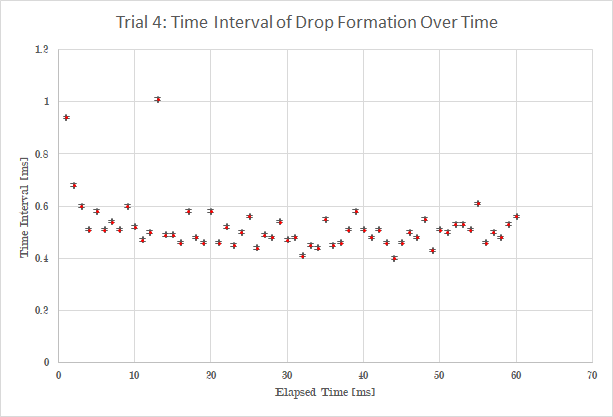
\includegraphics[width=\linewidth]{sink4.png}
  \captionof{figure}{sink4}
  \label{fig:test2}
\end{minipage}
\end{figure}

% plots 3 and 4
\begin{figure}[H]
\centering
\begin{minipage}{.5\textwidth}
  \centering
  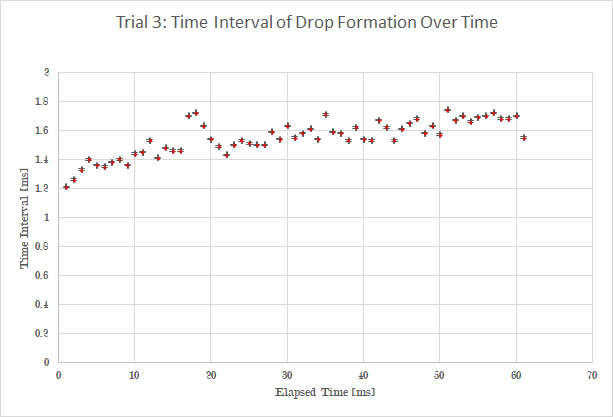
\includegraphics[width=\linewidth]{sink3.png}
  \captionof{figure}{sink3}
  \label{fig:test1}
\end{minipage}%
\begin{minipage}{.5\textwidth}
  \centering
  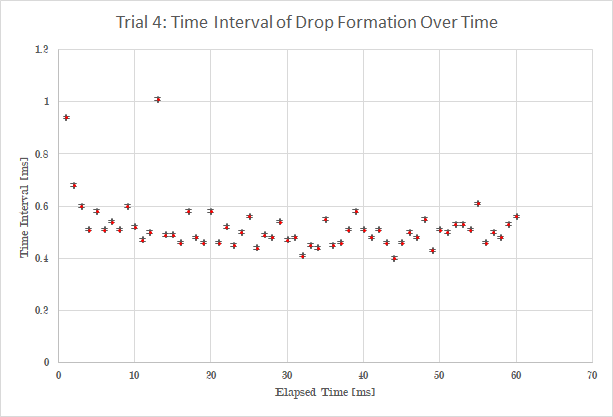
\includegraphics[width=\linewidth]{sink4.png}
  \captionof{figure}{sink4}
  \label{fig:test2}
\end{minipage}
\end{figure}

% plots 5 and 6
\begin{figure}[H]
\centering
\begin{minipage}{.5\textwidth}
  \centering
  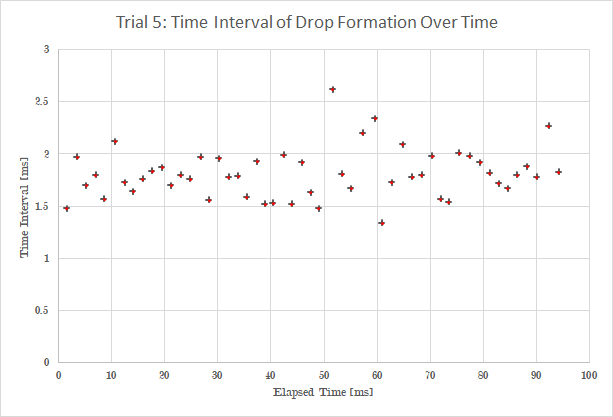
\includegraphics[width=\linewidth]{sink5.png}
  \captionof{figure}{sink5}
  \label{fig:test1}
\end{minipage}%
\begin{minipage}{.5\textwidth}
  \centering
  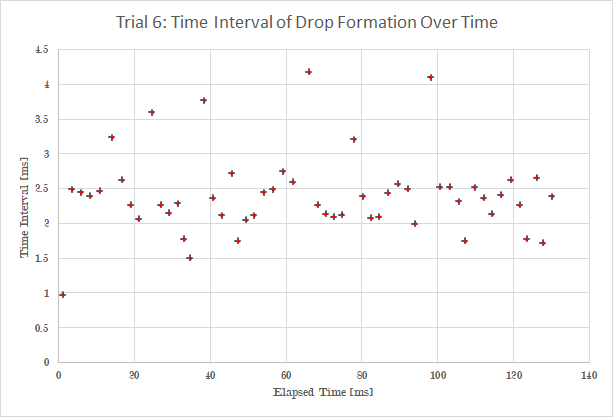
\includegraphics[width=\linewidth]{sink6.png}
  \captionof{figure}{sink6}
  \label{fig:test2}
\end{minipage}
\end{figure}

\section{Sources of Error}
%Discuss the radius/seperation
%Discuss the equipment heating
\qq 

\section{Conclusion}
%Brief summary, discussion of results and theory
\qq 

\section{Appendices}

\subsection{Appendix A: Data}

\subsection{Appendix B: Source Code}

\subsubsection{Error Propagation and Data Processing}

\end{document}
